\documentclass[]{article}
\usepackage[left=1in,top=1in,right=1in,bottom=1in]{geometry}


%%%% more monte %%%%
\usepackage{wrapfig}
% thispagestyle{empty}
% https://stackoverflow.com/questions/2166557/how-to-hide-the-page-number-in-latex-on-first-page-of-a-chapter
\usepackage{color}
% \usepackage[table]{xcolor} % are they using color?

% \definecolor{WSU.crimson}{HTML}{981e32}
% \definecolor{WSU.gray}{HTML}{5e6a71}

% \definecolor{shadecolor}{RGB}{248,248,248}
\definecolor{WSU.crimson}{RGB}{152,30,50} % use http://colors.mshaffer.com to convert from 981e32
\definecolor{WSU.gray}{RGB}{94,106,113}

%%%%%%%%%%%%%%%%%%%%%%%%%%%%

\newcommand*{\authorfont}{\fontfamily{phv}\selectfont}
\usepackage{lmodern}


  \usepackage[T1]{fontenc}
  \usepackage[utf8]{inputenc}




\usepackage{abstract}
\renewcommand{\abstractname}{}    % clear the title
\renewcommand{\absnamepos}{empty} % originally center

\renewenvironment{abstract}
 {{%
    \setlength{\leftmargin}{0mm}
    \setlength{\rightmargin}{\leftmargin}%
  }%
  \relax}
 {\endlist}

\makeatletter
\def\@maketitle{%
  \pagestyle{empty}
  \newpage
%  \null
%  \vskip 2em%
%  \begin{center}%
  \let \footnote \thanks
    {\fontsize{18}{20}\selectfont\raggedright  \setlength{\parindent}{0pt} \@title \par}%
}
%\fi
\makeatother









\title{\textbf{\textcolor{WSU.crimson}{Denzel Washington Consistently
Displays Excellence in Acting}}  }
 

%  

% \author{ \Large true \hfill \normalsize \emph{} }
\author{\Large Rachel
Judd\vspace{0.05in} \newline\normalsize\emph{Washington State University
Vancouver}  }


\date{April 25, 2021}
\setcounter{secnumdepth}{3}

\usepackage{titlesec}
% See the link above: KOMA classes are not compatible with titlesec any more. Sorry.
% https://github.com/jbezos/titlesec/issues/11
\titleformat*{\section}{\bfseries}
\titleformat*{\subsection}{\bfseries\itshape}
\titleformat*{\subsubsection}{\itshape}
\titleformat*{\paragraph}{\itshape}
\titleformat*{\subparagraph}{\itshape}

% https://code.usgs.gov/usgs/norock/irvine_k/ip-092225/


%\titleformat*{\section}{\normalsize\bfseries}
%\titleformat*{\subsection}{\normalsize\itshape}
%\titleformat*{\subsubsection}{\normalsize\itshape}
%\titleformat*{\paragraph}{\normalsize\itshape}
%\titleformat*{\subparagraph}{\normalsize\itshape}

% https://tex.stackexchange.com/questions/233866/one-column-multicol-environment#233904
\usepackage{environ}
\NewEnviron{auxmulticols}[1]{%
  \ifnum#1<2\relax% Fewer than 2 columns
    %\vspace{-\baselineskip}% Possible vertical correction
    \BODY
  \else% More than 1 column
    \begin{multicols}{#1}
      \BODY
    \end{multicols}%
  \fi
}





\usepackage{natbib}
\setcitestyle{aysep={}} %% no year, comma just year
% \usepackage[numbers]{natbib}
\bibliographystyle{./../00-latex-setup/biblio/ormsv080.bst}



\usepackage[strings]{underscore} % protect underscores in most circumstances




\newtheorem{hypothesis}{Hypothesis}
\usepackage{setspace}


%%%%%%%%%%%%%%%%%%%%%%%%%%%%%%%%%%%%%%%%%%%%%%%%%%%%%
%%% MONTE ADDS %%%

\usepackage{fancyhdr} % fancy header 
\usepackage{lastpage} % last page 

\usepackage{multicol}


\usepackage{etoolbox}
\AtBeginEnvironment{quote}{\singlespacing\small}
% https://tex.stackexchange.com/questions/325695/how-to-style-blockquote


\usepackage{soul}			%% allows strike-through
\usepackage{url}			%% fixes underscores in urls
\usepackage{csquotes}		%% allows \textquote in references
\usepackage{rotating}		%% allows table and box rotation
\usepackage{caption}		%% customize caption information
\usepackage{booktabs}		%% enhance table/tabular environment
\usepackage{tabularx}		%% width attributes updates tabular
\usepackage{enumerate}		%% special item environment
\usepackage{enumitem}		%% special item environment

\usepackage{lineno}		%% allows linenumbers for editing using \linenumbers
\usepackage{hanging}


\usepackage{mathtools}  	%% also loads amsmath
\usepackage{bm}		%% bold-math
\usepackage{scalerel}	%% scale one element (make one beta bigger font)

\newcommand{\gFrac}[2]{ \genfrac{}{}{0pt}{1}{{#1}}{#2} }

\newcommand{\betaSH}[3]{  \gFrac{\text{\tiny #1}}{{\text{\tiny #2}}}\hat{\beta}_{\text{#3}}   }
\newcommand{\betaSB}[3]{              ^{\text{#1}} _{\text{#2}} \bm{\beta} _{\text{#3}}                   }  %% bold
\newcommand{\bigEQ}{  \scaleobj{1.5}{{\ }= } }
\newcommand{\bigP}[1]{  \scaleobj{1.5}{#1 } }





\usepackage{endnotes}  % he already does this ...
\renewcommand{\enotesize}{\normalsize}
% https://tex.stackexchange.com/questions/99984/endnotes-do-not-be-superscript-and-add-a-space
\renewcommand\makeenmark{\textsuperscript{[\theenmark]}} % in brackets %
% https://tex.stackexchange.com/questions/31574/how-to-control-the-indent-in-endnotes
\patchcmd{\enoteformat}{1.8em}{0pt}{}{}

\patchcmd{\theendnotes}
  {\makeatletter}
  {\makeatletter\renewcommand\makeenmark{\textbf{[\theenmark]} }}
  {}{}



% https://tex.stackexchange.com/questions/141906/configuring-footnote-position-and-spacing

\addtolength{\footnotesep}{5mm} % change to 1mm

\renewcommand{\thefootnote}{\textbf{\arabic{footnote}}}
\let\footnote=\endnote
%\renewcommand*{\theendnote}{\alph{endnote}}
%\renewcommand{\theendnote}{\textbf{\arabic{endnote}}}


\renewcommand*{\notesname}{ENDNOTES}

\makeatletter
\def\enoteheading{\section*{\notesname
  \@mkboth{\MakeUppercase{\notesname}}{\MakeUppercase{\notesname}}}%
  \mbox{}\par\vskip-2.3\baselineskip\noindent\rule{.5\textwidth}{0.4pt}\par\vskip\baselineskip}
\makeatother


\renewcommand*{\contentsname}{TABLE OF CONTENTS}

\renewcommand*{\refname}{REFERENCES}


%\usepackage{subfigure}
\usepackage{subcaption}

\captionsetup{labelfont=bf}  % Make Table / Figure bold

%%% you could add elements here ... monte says .... %%%
%\usepackage{mypackageForCapitalH}


%%%%%%%%%%%%%%%%%%%%%%%%%%%%%%%%%%%%%%%%%%%%%%%%%%%%%

% set default figure placement to htbp
\makeatletter
\def\fps@figure{htbp}
\makeatother


% move the hyperref stuff down here, after header-includes, to allow for - \usepackage{hyperref}

\makeatletter
\@ifpackageloaded{hyperref}{}{%
\ifxetex
  \PassOptionsToPackage{hyphens}{url}\usepackage[setpagesize=false, % page size defined by xetex
              unicode=false, % unicode breaks when used with xetex
              xetex]{hyperref}
\else
  \PassOptionsToPackage{hyphens}{url}\usepackage[draft,unicode=true]{hyperref}
\fi
}

\@ifpackageloaded{color}{
    \PassOptionsToPackage{usenames,dvipsnames}{color}
}{%
    \usepackage[usenames,dvipsnames]{color}
}
\makeatother
\hypersetup{breaklinks=true,
            bookmarks=true,
            pdfauthor={Rachel Judd (Washington State University
Vancouver)},
             pdfkeywords = {Denzel Washington;Will Smith; excellence in
acting},  
            pdftitle={Denzel Washington Consistently Displays Excellence
in Acting},
            colorlinks=true,
            citecolor=blue,
            urlcolor=blue,
            linkcolor=magenta,
            pdfborder={0 0 0}}
\urlstyle{same}  % don't use monospace font for urls

% Add an option for endnotes. -----

%
% add tightlist ----------
\providecommand{\tightlist}{%
\setlength{\itemsep}{0pt}\setlength{\parskip}{0pt}}

% add some other packages ----------

% \usepackage{multicol}
% This should regulate where figures float
% See: https://tex.stackexchange.com/questions/2275/keeping-tables-figures-close-to-where-they-are-mentioned
\usepackage[section]{placeins}



\pagestyle{fancy}   
\lhead{\textcolor{WSU.crimson}{\textbf{ Denzel Washington Consistently
Displays Excellence in Acting }}}
\chead{}
\rhead{\textcolor{WSU.gray}{\textbf{  Page\ \thepage\ of\ \protect\pageref{LastPage} }}}
\lfoot{}
\cfoot{}
\rfoot{}


\begin{document}
	
% \pagenumbering{arabic}% resets `page` counter to 1 
%    

% \maketitle

{% \usefont{T1}{pnc}{m}{n}
\setlength{\parindent}{0pt}
\thispagestyle{plain}
{\fontsize{18}{20}\selectfont\raggedright 
\maketitle  % title \par  

}

{
   \vskip 13.5pt\relax \normalsize\fontsize{11}{12} 
   
\textbf{\authorfont Rachel Judd} \hskip 15pt \emph{\small Washington
State University Vancouver}   

}

}








\begin{abstract}

    \hbox{\vrule height .2pt width 39.14pc}

    \vskip 8.5pt % \small 

\noindent Denzel Washington is a better actor than Will Smith. This is
seen through ratings, votes, millions of dollars earned, and the depth
and breadth of genres acted in. In each of these categories, Washington
displays consistency and excellence in acting.


\vskip 8.5pt \noindent \textbf{\underline{Keywords}:} Denzel
Washington;Will Smith; excellence in acting \par

    




    
    \hbox{\vrule height .2pt width 39.14pc}
    \vskip 5pt 
    \hfill \textbf{\textcolor{WSU.gray}{ April 25, 2021 } }
    \vskip 5pt 
    
\end{abstract}


\vskip -8.5pt



 % removetitleabstract

\noindent  

\begin{figure}[!ht]
 \label{fig:one-graphic}
%% figures have hrule, tables have hline
    \begin{center}
        \scalebox{1.00}{    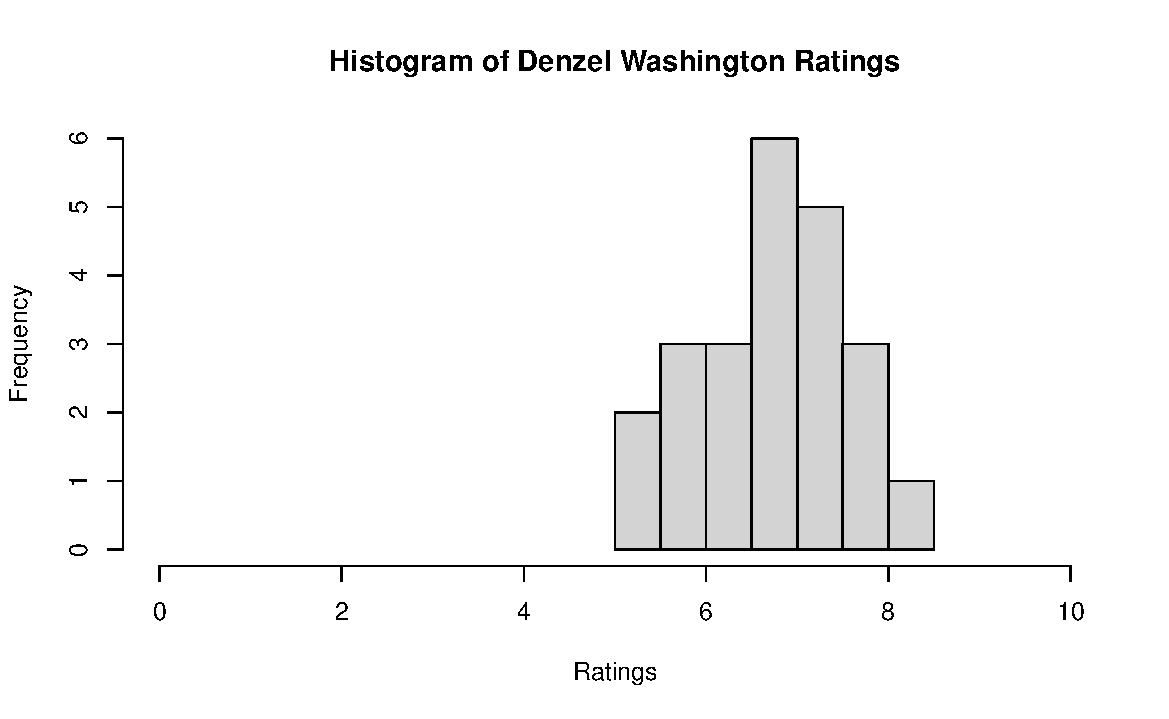
\includegraphics[trim = 0 15mm 0 15mm,clip,width=\textwidth]{figures/DWRatingPortrait.pdf} }
    \end{center}
    \hrule
      \vspace{2mm}
    \caption{ \textbf{Denzel Washington's ratings are clustered in the higher end of the rating scale:} \newline \footnotesize{ This graph shows the frequency of ratings for Denzel Washington's movies.  \newline \newline  The lowest rating is 5.0 while the highest rating is 8.5, with a median of 6.85. }  }
    \vspace{2mm}
    \hrule
\end{figure}

\newpage
\section{Introduction}
\label{sec:intro}

\doublespacing

There are several ways to measure success as an actor, including votes,
millions earned, ratings, metacritic ratings, and the breadth and depth
of genres in which the actor has acted. The votes show how well-liked
the actor's movies are, with more votes reflecting superior acting
performance. The millions of dollars each movie earns is an important
measure of an actor's success. Higher earnings reflect better
performance. High ratings also reflect excellent acting. The ability to
act in mulitiple genres demonstrates flexibility and high level of
skill.

Denzel Washington has demonstrated excellence in acting through
consistent ratings, high earnings, high numbers of votes, and a good
depth and breadth of acting experience. In each of these dimensions,
Washington has shown that he is superior to other actors such as Will
Smith.

\newpage
\section{ Comparison to Will Smith}
\label{sec:da}

Denzel Washington acts in consistently longer films than Will Smith. The
longest film Washington has acted in is 202 minutes, 45 minutes longer
than Smith's longest film. The shortest film Washington has acted in is
60 minutes long, 13\% longer than Smith's shortest film. Washington's
median film length is 118 minutes, 11\% longer than Smith's median film
length.

Washington's films have received higher ratings than Smith's. The lowest
rating Washington has received is 5.0, which is 54\% higher than Smith's
lowest rating of 2.3. The highest rating Washington has received is 8.5
and he has a median rating of 6.85, 8\% higher than Smith's median
rating. These consistently high ratings show superior acting
performance.

Washington's films have also received higher metacritic ratings than
Smith's films. The lowest metacritic rating Washington has received is
30, 50\% higher than Smith's lowest. The highest metacritic rating
Washington has received is 79, a higher score than Smith's highest
metacritic rating. Washington has a mean metacritic rating of 61, which
is 15\% higher than Smith's mean metacritic rating.

The lowest number of votes Washington's films have gotten is 330, 90\%
more than the lowest number of votes one of Smith's films has received
(34 votes). The highest number of votes Washington's movies have earned
is 383,980, with a median of 74,561. Smith's median number of votes is
56,408, 24\% less than Washington's median.

The highest Washington's films have earned is 120.09 million dollars
(standardized to 2000). The lowest one of his films has ever earned is
0.2766 million dollars, 95\% more than the lowest Smith's films have
earned. The median earnings of Washington's films is 52.45 million
dollars, 6\% more than the median of Smith's film's earnings.

Washington has acted in 16 different genres, compared to Smith's 18
genres. The majority (71\%) of Washington's movies are drama, with crime
the second most acted in genre at 34\%. By specializing in drama and
crime, Washington has been able to strengthen his performance in two
specific genres while maintaining the versatility to act in many
different genres.

\section{ Conclusion}
\label{sec:conclusion}

The assessment of excellence in acting requires multiple measures
including votes received, ratings, metacritic ratings, millions of
dollars earned, and the depth and breadth of acting experience. These
measures work together to show how well-liked the actor's movies are,
the monetary value of these movies, and the actor's flexibility and
height of skill. On each of these dimensions, Denzel Washington has
shown himself superior to actors like Will Smith, consistently
displaying excellence in acting.




%% appendices go here!


\newpage
\theendnotes

%%%%%%%%%%%%%%%%%%%%%%%%%%%%%%%%%%%  biblio %%%%%%%%
\newpage
\begin{auxmulticols}{1}
\singlespacing 
\bibliography{./../00-latex-setup/biblio/master.bib}

%%%%%%%%%%%%%%%%%%%%%%%%%%%%%%%%%%%  biblio %%%%%%%%
\end{auxmulticols}

\newpage
{
\hypersetup{linkcolor=black}
\setcounter{tocdepth}{3}
\tableofcontents
}



\end{document}